\setAuthor{Oleg Košik}
\setRound{lõppvoor}
\setYear{2007}
\setNumber{G 6}
\setDifficulty{7}
\setTopic{Gaasid}

\prob{Gaasid}
\begin{wrapfigure}[8]{r}{0.2\textwidth}
	\begin{center}
		\vspace{-20pt}
		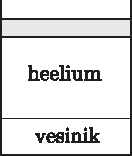
\includegraphics[width=0.95\linewidth]{2007-v3g-06-yl}
	\end{center}
\end{wrapfigure}
Isoleeritud silindrilises anumas vabalt liikuva koormise all on vesinik ja heelium, mis on teineteisest eraldatud vabalt liikuva ja aeglaselt soojust juhtiva õhukese vaheseinaga (vt. joonist). Alguses on gaaside temperatuurid võrdsed, kusjuures vesinik hõlmab heeliumist 3 korda väiksema ruumala. Vesinikule anti teatud soojushulk, mille tulemusena nihkus koormis $d_1 = \SI{5,5}{cm}$ võrra ülespoole. Pika aja möödudes täheldati, et koormis nihkus veel. Mis suunas ja kui palju see nihkus? Gaasid lugeda ideaalseteks. Vesiniku soojusmahtuvus konstantsel rõhul on $C\idx{PH_2} = 7R/2$ ning heeliumil $C\idx{PHe} = 5R/2$.

\hint
Esialgu on vesinik teatud temperatuurivahe võrra soojem kui heelium, kuid pika aja möödudes on mõlemad soojuslikus tasakaalus. Koormise nihe ongi põhjustatud gaaside soojenemisest tulenevast paisumisest.

\solu
Kogu protsessi jooksul on mõlema gaasi rõhud võrdsed ja konstantsed. Olgu vesiniku moolide arv $n_0$. Kuna alguses on ka temperatuurid võrdsed, siis valemi $n = \frac{pV}{RT}$ põhjal näeme, et heeliumi moolide arv peab olema $3n_0$. Konstantsel rõhul avaldub molaarne erisoojus kui $C_P = \left(\frac{i}{2} + 1\right) R$ (see valem on tuletatav ka teistest rohkem tuntud valemitest). Vesinik on kaheaatomiline gaas, heelium aga üheaatomiline, seega $i\idx{H_2} = 5$, $i\idx{He} = 3$ ning järelikult $C\idx{PH_2} = 7/2R$ ja $C\idx{PHe} = 5/2R$.

Omandagu vesinik vahetult peale soojendamist temperatuuri, mis on algtemperatuurist $\Delta T_1$ võrra kõrgem ning olgu terve süsteemi tasakaaluline lõpptemperatuur algtemperatuurist $\Delta T_2$ võrra suurem. Heelium saab temperatuuride ühtlustumise ajal soojushulga $3n_0C\idx{PHe}\Delta T_2$, mis peab võrduma vesiniku poolt ära antava soojushulgaga:
\[
n_0C\idx{PH_2} (\Delta T_1 - \Delta T_2) = 3n_0C\idx{PHe}\Delta T_2,
\]
ehk
\[
\frac{7}{2} (\Delta T_1 - \Delta T_2) = 3 \cdot \frac{5}{2} \Delta T_2,
\]
kust
\[
\Delta T_2 = \frac{7}{22} \Delta T_1.
\]
Kuna protsess on isobaariline ja nii alguses kui ka lõpus on gaaside temperatuurid võrdsed, siis kehtivad võrdused $pV\idx{H_2} = n\idx{H_2}RT$, $p(V\idx{H_2} + V\idx{He}) = (n\idx{He} + n\idx{H_2} )RT = 4n_0RT$. Siit tulenevalt kehtib ka
\[
p\Delta V\idx{H_2} = n_0R\Delta T_1,
\]
\[
p\Delta (V\idx{H_2} + V\idx{He}) = 4n_0R\Delta T2.
\]
Järelikult
\[
\frac{d_{2}}{d_{1}}=\frac{\Delta\left(V\idx{H_{2}}+V\idx{H e}\right)}{\Delta V\idx{H_{2}}}=\frac{4 \Delta T_{2}}{\Delta T_{1}}=\frac{28}{22}.
\]
Seega lõpus on koormus algusega võrreldes $d_2 = \frac{28}{22} d_1 = \SI{7}{cm}$ kõrgemal, järelikult ta nihkub täiendavalt $\Delta d = d_2 - d_1 = \SI{1,5}{cm}$ ülespoole.
\probend